
Streamers are long, dense structures of gas acting as pathways for material to move from the surrounding envelope to the disk \citep{Heigl}. The Early Planet Formation in Embedded Disks (eDIsk) study of IRS 63 first proposed a streamer based on observations of two molecular tracers \citep{Flores}. Following this, a study by \cite{Podio} presented molecular-line emission, tracing the streamer to study its impact on the southeast disk side, as shown in Figure \ref{fig: streamer}. 


 During the analysis of \bfive with \texttt{robust = 0.5}, a small number of polarization vectors were found that satisfied the reliability criteria but were located outside of the main group of vectors. These vectors are shown in red in Figure \ref{fig: Band5_robust05}. Additionally, the vectors have similar orientations, suggesting that the emission is from the same source. \question{Is this true or useful at all?} Comparing their location with the observations from \cite{Podio}, the red polarization vectors are located in the same region as the streamer. The bounds of Figure \ref{fig: Band5_robust05} are overlaid on Figure \ref{fig: streamer} to show the similarity between the two observations. 


 
The observed polarization emission in the region of the streamer is unlikely to be a result of dust self-scattering. The streamer is located outside of the dense regions of the disk, where dust grains are expected to be smaller and therefore less efficient at scattering. Other polarization mechanisms cannot be ruled out. However, polarization from magnetically aligned grains is a possible explanation for the emission. If the polarization is caused by magnetic alignment, the orientation of the magnetic field can be determined since the long axes of grains tend to align perpendicular to the magnetic field \citep{Lazarian}. The polarization vectors of the streamer are therefore rotated by $90^\circ$ to show the magnetic field orientation. Since the polarization vectors do not have a direction, these observations cannot determine whether the magnetic field is oriented towards or away from the disk, or determine the direction of the flow of material.




Observational studies on the relationship between streamers and magnetic fields are uncommon, but some examples include SVS 13A \citep{Cort} and HOPS-182 \citep{Huang_2026}. This observation in IRS 63 may indicate a connection between the streamer and the magnetic field, providing an additional opportunity to study this relationship. However, only a few polarization vectors were detected in the streamer, and further investigation is beyond the scope of this thesis.






 
\begin{figure}[htbp]
  \centering
  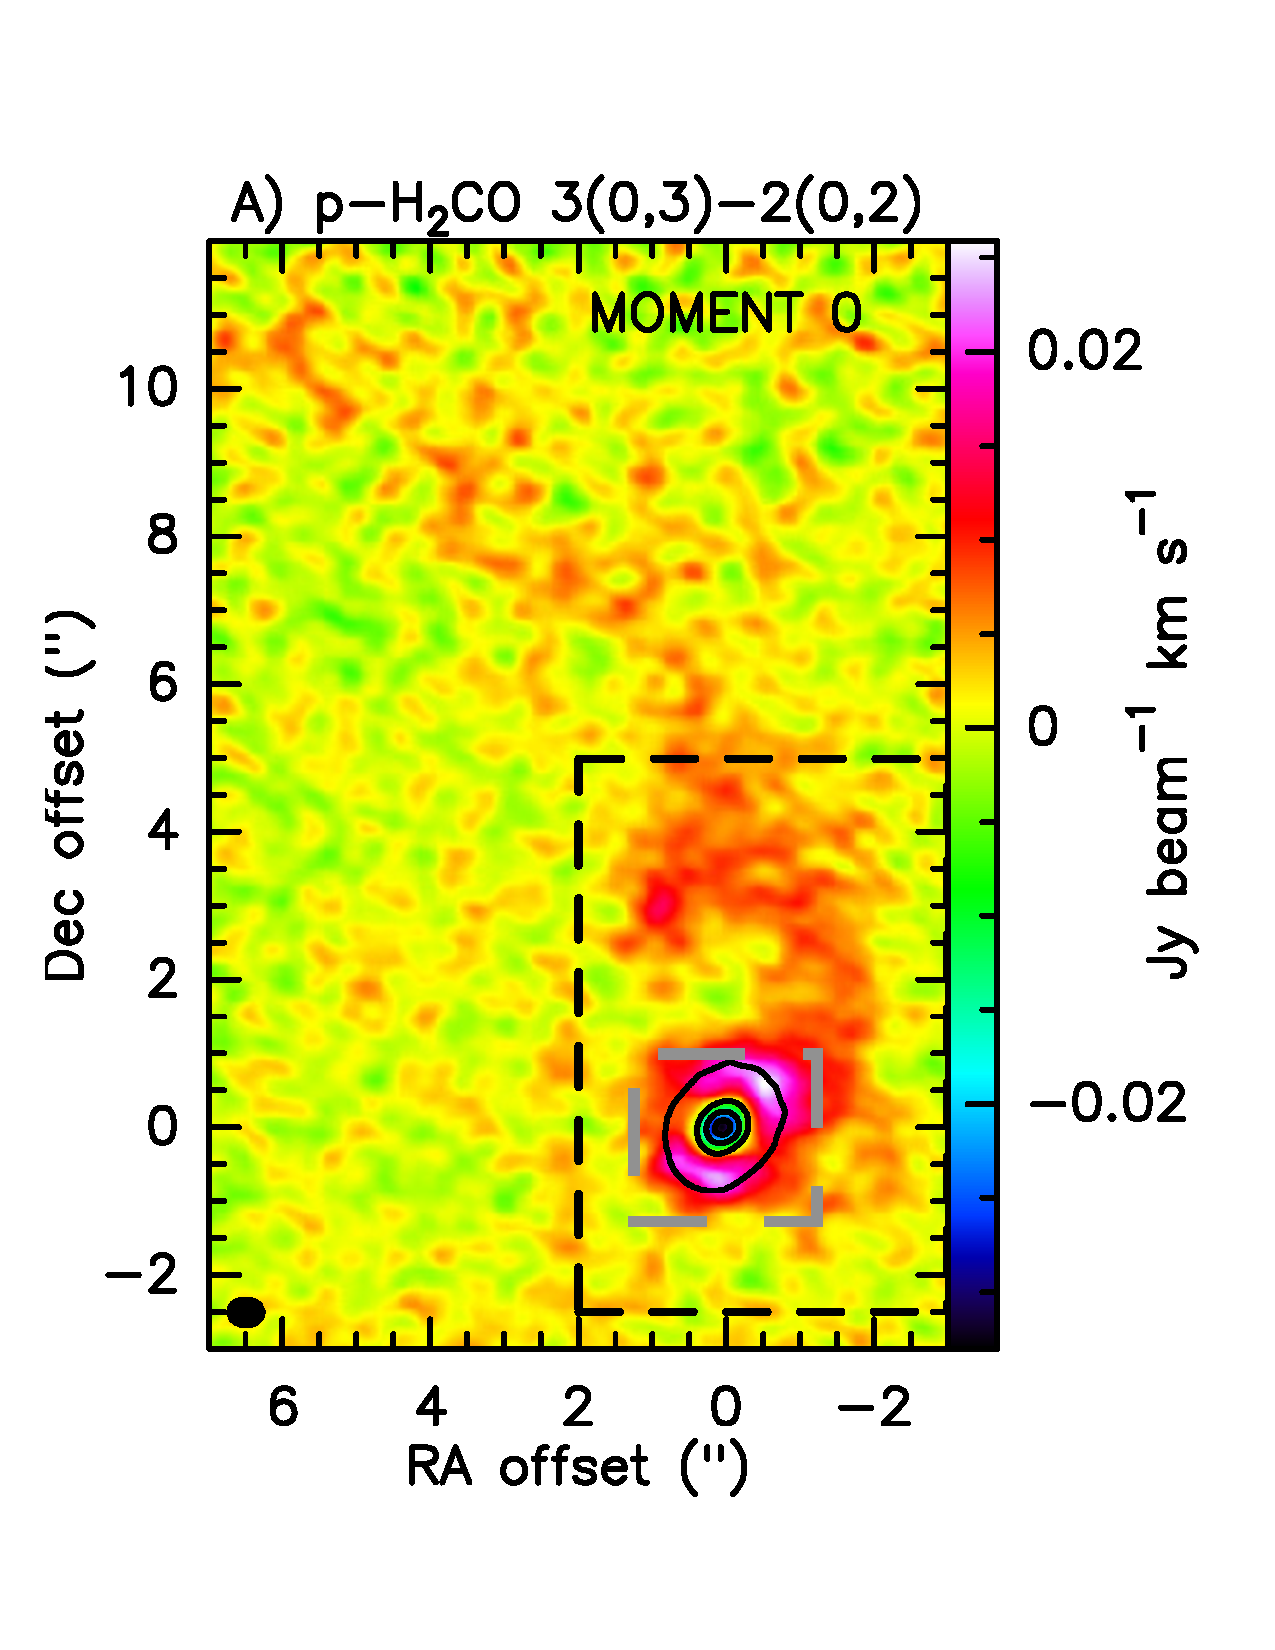
\includegraphics[width=0.5\textwidth]{WRITEUP_AND_IMAGES/IMAGES/WRITEUP/NOTMINE/aa50742-24-fig1_v2.pdf}
  \caption{Moment 0 map of p-H$_2$CO $3(0,3)-2(0,2)$ from IRS 63, showing the disk and the streamer in the southeast region. The grey dashed box is the region shown in Figure \ref{fig: Band5_robust05}. Image from \cite{Podio}. \permission{ask for permission.} }
  \label{fig: streamer}
\end{figure}